   
\documentclass[11pt]{article}
\usepackage{amsmath,amsthm,verbatim,amssymb,amsfonts,amscd, graphicx}
\usepackage{graphicx}
\usepackage{float}
\topmargin0.0cm
\headheight0.0cm
\headsep0.0cm
\oddsidemargin0.0cm
\textheight23.0cm
\textwidth16.5cm
\footskip1.0cm
\theoremstyle{plain}
\newtheorem{theorem}{Theorem}
\newtheorem{corollary}{Corollary}
\newtheorem{lemma}{Lemma}
\newtheorem{proposition}{Proposition}
\newtheorem*{surfacecor}{Corollary 1}
\newtheorem{conjecture}{Conjecture} 
\newtheorem{question}{Question} 
\theoremstyle{definition}
\newtheorem{definition}{Definition}

\begin{document}
\title{CS 5220\\ Project 1 - Matrix Multiplication}
\author{Weici Hu(wh343)\\ Sheroze Sheriffdeen(mss385)\\ Qinyu Wang(qw78)}
\maketitle

\section{Introduction}
In this project, we tried several methods to fine-tune square matrix multiplication.
Based on the \texttt{dgemm\_blocked.c}, we tried unrolling index, modifying loop sequence to take advantage of SSE, and experimenting with different optimization flags.

\section{Optimization}
\subsection{Block Multiplication with Multiple Block Sizes}
\subsubsection{Approach}
Working off of \texttt{dgemm\_blocked.c}, we tried different block sizes to examine the performance changes. 
\subsubsection{Results}
Figure \ref{pow_2_blocks} shows the performance of different approaches with various block sizes. (block sizes are a multiple of 2). The performance gain for varying block sizes is not immense but a block size of 64 performs better than other block sizes. \\

\begin{figure}[H]
    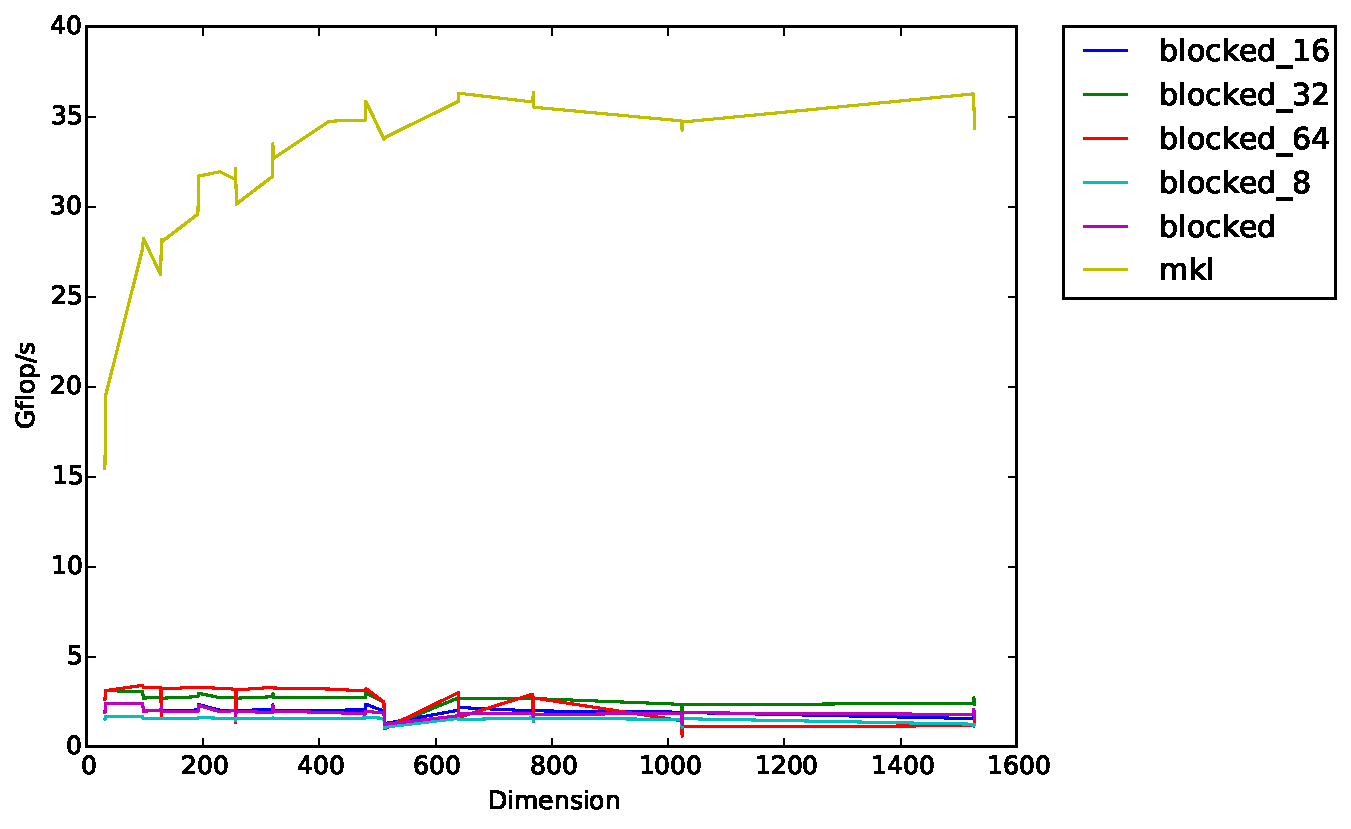
\includegraphics[width=0.9\textwidth]{timing_block_size_changes.pdf}
    \caption{Block size variation}
    \label{pow_2_blocks}
\end{figure} 

In addition, we attempted block sizes that are not a multiple of 2. Figure \ref{odd_blocks} is the comparison of the performance against a block size of 64.\\
\begin{figure}[H]
    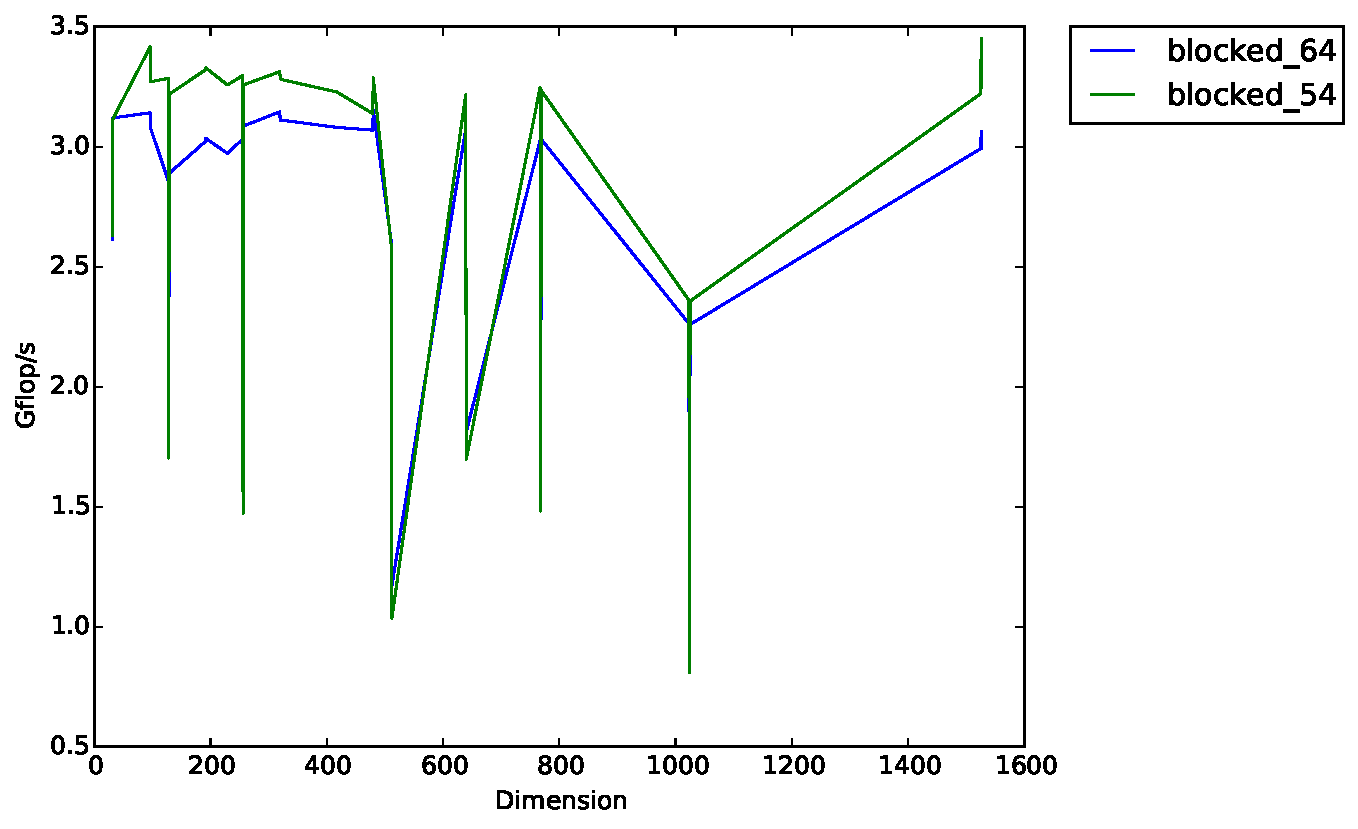
\includegraphics[width=0.9\textwidth]{timing_54_64.pdf}
    \caption{Block size variation}
    \label{odd_blocks}
\end{figure} 


\subsection{Block Multiplication with Manual Loop Unrolling}
\subsubsection{Approach}
In this approach, we manually unrolled 4 computations in the inner most loop of the matrix multiplication of a block. 
\subsubsection{Results}
Figure \ref{unrolled_vs_regular} compares the performance of the unrolled blocked version against the vanilla blocked approach. The unrolled versions clearly perform better than the original blocked approach but not by much. 
\begin{figure}[H]
    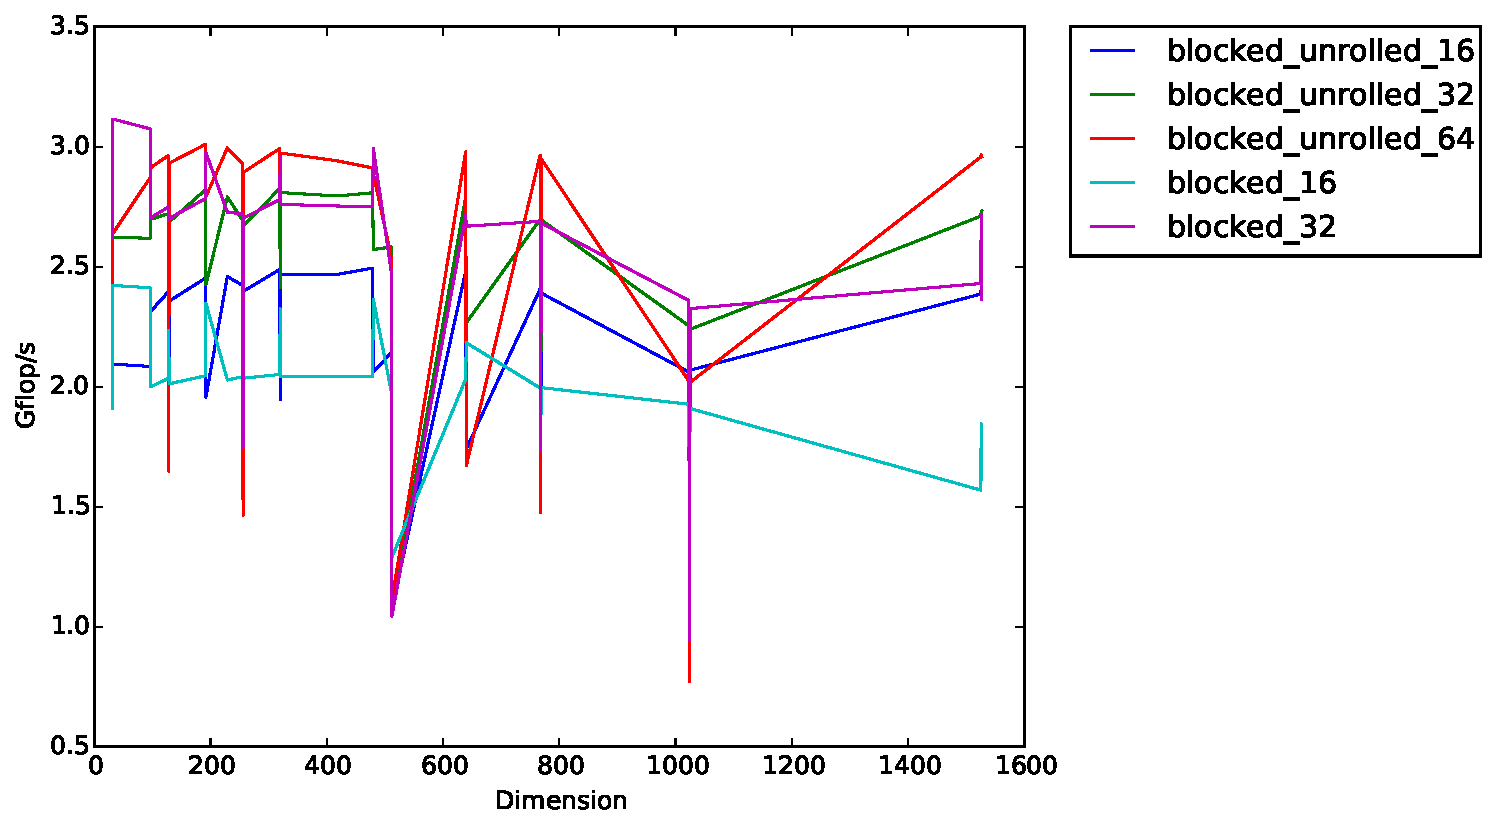
\includegraphics[width=0.9\textwidth]{timing_unrolled_vs_nonunrolled.pdf}
    \caption{Unrolled blocks vs regular blocks}
    \label{unrolled_vs_regular}
\end{figure} 

\subsection{Compiler Optimization Flags}
\subsubsection{Approach}
Using the blocked approach as a baseline, we examine the effect of various compiler flags on the multiplication.
\subsubsection{Results}
Figure \ref{all_optimized_blocked} shows the performance of blocked multiplication with the flags, \texttt{-march=native -funroll-loops -ftree-vectorize}.
\begin{figure}[H]
    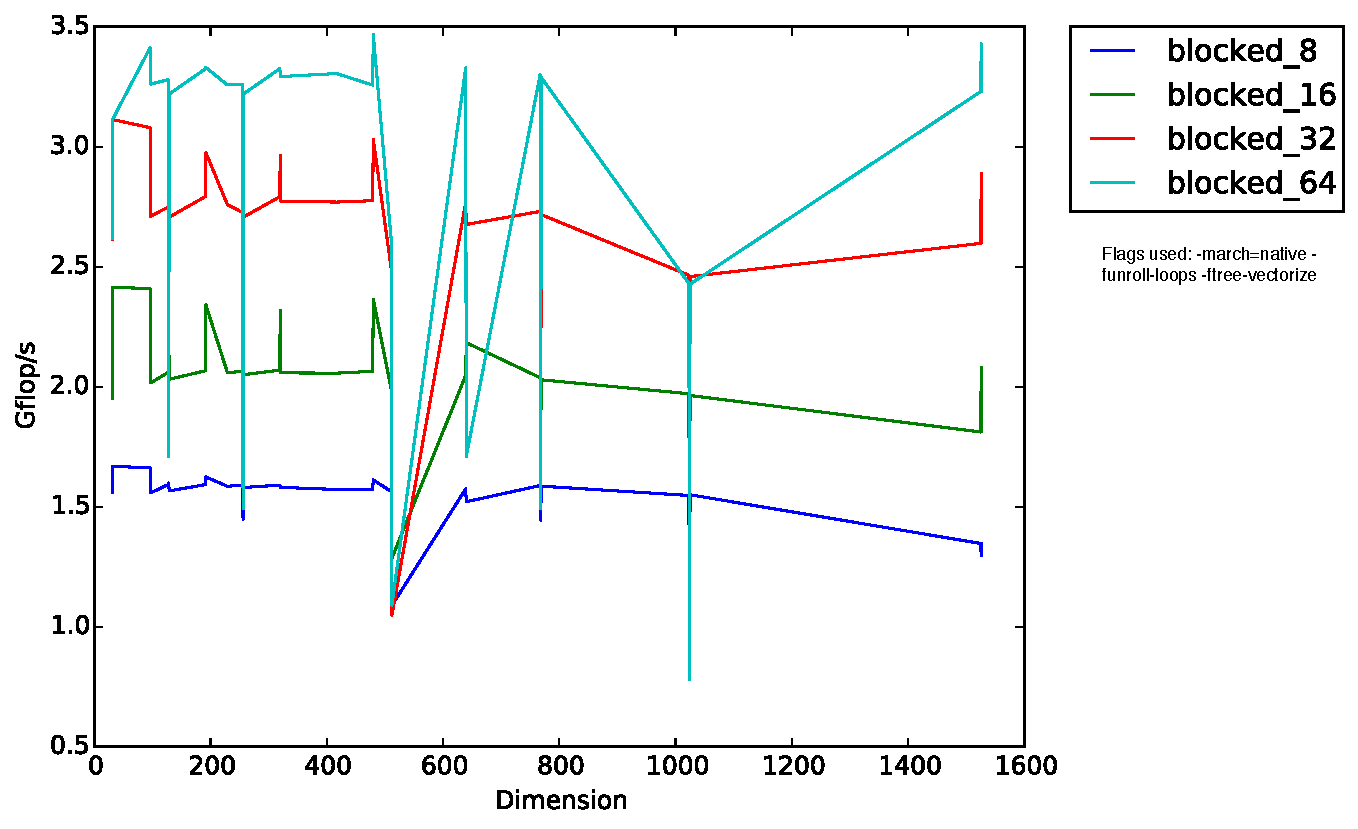
\includegraphics[width=0.9\textwidth]{timing_flags_blocked.pdf}
    \caption{Compiler flags \texttt{-march=native -funroll-loops -ftree-vectorize}}
    \label{all_optimized_blocked}
\end{figure} 


\subsection{Loop reordering}
\subsubsection{Approach}
\subsubsection{Results}


\subsection{AVX Instructions}
\subsubsection{Approach}
//Describe what we did here.
\subsubsection{Results}
//Add graphs here.



\section{Next Steps}
\subsection{Copy Optimization}





 
 
\end{document}